\chapter{हृदय और रक्त}\label{ch:g4:heart-and-blood}

अपनी \omterm{def:g1:my-body:joint}{कलाई} के भीतरी हिस्से पर, अँगूठे के ठीक नीचे, दो उँगलियाँ रखो
--- अँगूठा नहीं --- और रुको। लो: एक छोटी, लगातार दस्तक, बार-बार, लगभग
हर सेकंड। यह दस्तक तुम्हारा \omterm{def:g4:heart-and-blood:heart}{हृदय} है, जो दूर से महसूस हो रहा है। वह
तुम्हारे जन्म से भी पहले से धड़क रहा है, और वही शरीर की पहुँचाने वाली
सेवा का इंजन है।

\section{रक्त, शरीर की पहुँचाने वाली सेवा}

\begin{proposition}[रक्त क्या ढोता है]\label{prop:g4:heart-and-blood:carries}
\emph{रक्त}\index{रक्त} वह तरल है जो शरीर के हर कोने तक पहुँचता है, और
वही शरीर का ढोने वाला है:
\begin{itemize}
  \item \omterm{def:g4:journey-of-food:tract}{छोटी आँत} से वह \emph{\omterm{def:g4:journey-of-food:digestion}{पोषक तत्व}} बटोरता है
        (\cref{prop:g4:journey-of-food:absorb});
  \item फेफड़ों से वह \emph{ऑक्सीजन} बटोरता है
        (\cref{prop:g4:breathing:exchange});
  \item और दोनों को शरीर के हर हिस्से तक पहुँचाता है --- \omterm{def:g3:bones-and-muscles:muscle}{पेशियों},
        मस्तिष्क, \omterm{def:g3:bones-and-muscles:skeleton}{हड्डियों}, \omterm{def:g1:the-five-senses:sense}{त्वचा} तक;
  \item लौटते समय वह कचरा उठा ले जाता है, और कार्बन डाइऑक्साइड को
        फेफड़ों तक पहुँचा देता है ताकि वह साँस के साथ बाहर निकल जाए।
\end{itemize}
\end{proposition}
\admitted

\begin{example}[एक चक्कर]\label{ex:g4:heart-and-blood:round}
\omterm{prop:g4:journey-of-food:absorb}{रक्त} की एक बूँद के पीछे चलो: फेफड़ों से गुज़रकर वह चटक लाल हो जाती है,
ऑक्सीजन से लदी हुई; \omterm{def:g4:heart-and-blood:heart}{हृदय} उसे बाहर भेजता है; दौड़ती \omterm{def:g1:my-body:parts}{टाँग} की \omterm{def:g3:bones-and-muscles:muscle}{पेशी} में वह
ऑक्सीजन और \omterm{def:g4:journey-of-food:digestion}{पोषक तत्व} सौंप देती है, कार्बन डाइऑक्साइड ले लेती है, और
गहरी पड़ जाती है; \omterm{def:g4:heart-and-blood:heart}{हृदय} पर लौटते ही उसे फेफड़ों में भेजा जाता है, जहाँ
वह उतारती और फिर से लादती है --- और बाहर निकल पड़ती है। एक पूरा चक्कर
मिनट भर से भी कम में हो जाता है।
\end{example}

\begin{definition}[रक्त वाहिकाएँ]\label{def:g4:heart-and-blood:vessels}
\omterm{prop:g4:journey-of-food:absorb}{रक्त} उन नलियों में सफ़र करता है जिन्हें \omterm{prop:g4:journey-of-food:absorb}{रक्त}
\emph{वाहिकाएँ}\index{रक्त वाहिका} कहते हैं: \omterm{def:g4:heart-and-blood:heart}{हृदय} से निकलती और उसमें
लौटती चौड़ी वाहिकाएँ, जो बँटते-बँटते महीन से महीन होती जाती हैं --- और
अंत में बाल जितनी पतली वाहिकाएँ शरीर के हिस्सों के बीच बुनी रहती हैं,
जहाँ सामान सौंपा जाता है। एक शरीर की वाहिकाओं को सिरे से सिरे तक जोड़
दिया जाए तो वे दसियों हज़ार किलोमीटर लंबी हो जाएँ।
\end{definition}

\begin{remark}[वाहिकाओं को देखना]\label{rem:g4:heart-and-blood:see}
अपनी \omterm{def:g1:my-body:joint}{कलाई} की भीतरी सतह देखो: \omterm{def:g1:the-five-senses:sense}{त्वचा} के नीचे नीली-सी लकीरें --- ये \omterm{def:g4:heart-and-blood:heart}{हृदय}
की ओर लौटती \omterm{def:g4:heart-and-blood:vessels}{रक्त वाहिकाएँ} हैं। छिला हुआ \omterm{def:g1:my-body:joint}{घुटना} इस जाल का दूसरा सिरा
दिखा देता है: सबसे पतले कट पर भी \omterm{prop:g4:journey-of-food:absorb}{रक्त} निकल आता है, क्योंकि सबसे महीन
\omterm{def:g4:heart-and-blood:vessels}{वाहिकाएँ} हर जगह हैं।
\end{remark}

\section{हृदय, वह पंप}

\begin{definition}[हृदय]\label{def:g4:heart-and-blood:heart}
\emph{हृदय}\index{हृदय} एक खोखली \omterm{def:g3:bones-and-muscles:muscle}{पेशी} है, लगभग अपने ही मालिक की मुट्ठी
जितनी बड़ी, जो छाती के बीच में \omterm{def:g3:bones-and-muscles:skeleton}{पसलियों} के पिंजरे के पीछे बैठी है। दबकर
--- यानी एक \emph{धड़कन}\index{धड़कन} से --- वह \omterm{prop:g4:journey-of-food:absorb}{रक्त} को \omterm{def:g4:heart-and-blood:vessels}{वाहिकाओं} में
आगे ठेलता है। उसके दो पक्ष हैं: दायाँ पक्ष \omterm{prop:g4:journey-of-food:absorb}{रक्त} को ऑक्सीजन लादने के
लिए \emph{फेफड़ों} तक पंप करता है; बायाँ पक्ष ऑक्सीजन से भरे \omterm{prop:g4:journey-of-food:absorb}{रक्त} को
\emph{पूरे शरीर} में पंप करता है।
\end{definition}

\begin{omfigure}
\begin{tikzpicture}[scale=0.95]
  % heart: two chambers schematic
  \draw[thick, fill=omThm!10] (0,0)
    .. controls (-1.5,0.9) and (-1.3,2.3) .. (-0.35,2.3)
    .. controls (-0.05,2.3) and (0.0,2.15) .. (0.0,2.05)
    .. controls (0.0,2.15) and (0.05,2.3) .. (0.35,2.3)
    .. controls (1.3,2.3) and (1.5,0.9) .. (0,0);
  \draw[thick] (0,2.05) -- (0,0.35);
  \node[font=\small, align=center] at (-0.55,1.45) {दायाँ\\ पक्ष};
  \node[font=\small, align=center] at (0.55,1.45) {बायाँ\\ पक्ष};
  % arrows: right side to lungs
  \draw[->, very thick, omDef] (-0.55,2.3) .. controls (-0.8,3.0)
    .. (-1.9,3.2)
    node[left, font=\small, omDef, align=center] {फेफड़ों को:\\ ऑक्सीजन लादो};
  \draw[->, very thick, omDef!50] (-3.0,2.2) .. controls (-2.0,2.0)
    .. (-1.15,1.6);
  \node[font=\small, omDef!80, align=center, left] at (-3.05,2.2)
    {शरीर से\\ वापस};
  % arrows: left side to body
  \draw[->, very thick, omThm] (0.55,2.3) .. controls (0.8,3.0)
    .. (1.9,3.2)
    node[right, font=\small, omThm, align=center] {पूरे शरीर को:\\ ऑक्सीजन पहुँचाओ};
  \draw[->, very thick, omThm!50] (3.0,2.2) .. controls (2.0,2.0)
    .. (1.15,1.6);
  \node[font=\small, omThm!80, align=center, right] at (3.05,2.2)
    {फेफड़ों से\\ वापस};
\end{tikzpicture}

{\small \omterm{def:g4:heart-and-blood:heart}{हृदय} के दोनों पक्ष: दायाँ पक्ष \omterm{prop:g4:journey-of-food:absorb}{रक्त} को ऑक्सीजन के लिए फेफड़ों
तक भेजता है; बायाँ पक्ष लदे हुए \omterm{prop:g4:journey-of-food:absorb}{रक्त} को पूरे शरीर में घुमाता है।}
\end{omfigure}

\begin{proposition}[नाड़ी]\label{prop:g4:heart-and-blood:pulse}
हर \omterm{def:g4:heart-and-blood:heart}{धड़कन} \omterm{def:g4:heart-and-blood:vessels}{वाहिकाओं} में \omterm{prop:g4:journey-of-food:absorb}{रक्त} की एक छोटी लहर दौड़ा देती है; \omterm{def:g1:my-body:joint}{कलाई} या गरदन
पर महसूस की जाए तो वही लहर \emph{नाड़ी}\index{नाड़ी} है। \omterm{prop:g4:heart-and-blood:pulse}{नाड़ी} गिनना
धड़कनें गिनना है: आराम में बच्चे के लिए मिनट में लगभग $80$ से $100$,
वयस्क के लिए $60$ से $80$ --- और मेहनत के दौरान इससे कहीं ज़्यादा।
\end{proposition}
\admitted

\begin{example}[हृदय टाँगों का साथ निभाता है]\label{ex:g4:heart-and-blood:effort}
दौड़ते समय तुम्हारी \omterm{def:g1:my-body:parts}{टाँगों} की \omterm{def:g3:bones-and-muscles:muscle}{पेशियाँ} \omterm{def:g4:journey-of-food:digestion}{पोषक तत्व} और ऑक्सीजन तेज़ी से
जलाती हैं; इसलिए पहुँचाने की रफ़्तार बढ़नी ही चाहिए। तो \omterm{def:g4:heart-and-blood:heart}{हृदय} तेज़
\emph{और} ज़ोर से धड़कता है --- दौड़ में बच्चे की \omterm{prop:g4:heart-and-blood:pulse}{नाड़ी} $150$ पार कर
सकती है --- और साथ ही साँस तेज़ होकर \omterm{prop:g4:journey-of-food:absorb}{रक्त} को फिर से लादती है
(\cref{ex:g4:breathing:running})। \omterm{def:g4:heart-and-blood:heart}{हृदय} और \omterm{def:g4:breathing:organs}{फेफड़े} एक ही आपूर्ति-शृंखला
के दो आधे हिस्से हैं।
\end{example}

\begin{method}[नाड़ी देखना]\label{met:g4:heart-and-blood:pulse}
\begin{enumerate}
  \item एक हाथ की हथेली ऊपर करो; दूसरे हाथ की दो उँगलियाँ \omterm{def:g1:my-body:joint}{कलाई} पर,
        अँगूठे के ठीक नीचे रखो --- अँगूठा कभी नहीं, क्योंकि उसकी
        अपनी एक छोटी \omterm{prop:g4:heart-and-blood:pulse}{नाड़ी} होती है;
  \item धीरे से दबाओ जब तक दस्तक महसूस न हो;
  \item एक मिनट तक दस्तकें गिनो (सेकंड वाली घड़ी मदद करती है);
  \item संख्या लिख लो, और साथ में यह भी कि शरीर उस समय क्या कर रहा था:
        आराम, चलना, या दौड़ के बाद।
\end{enumerate}
\end{method}

\begin{omfigure}
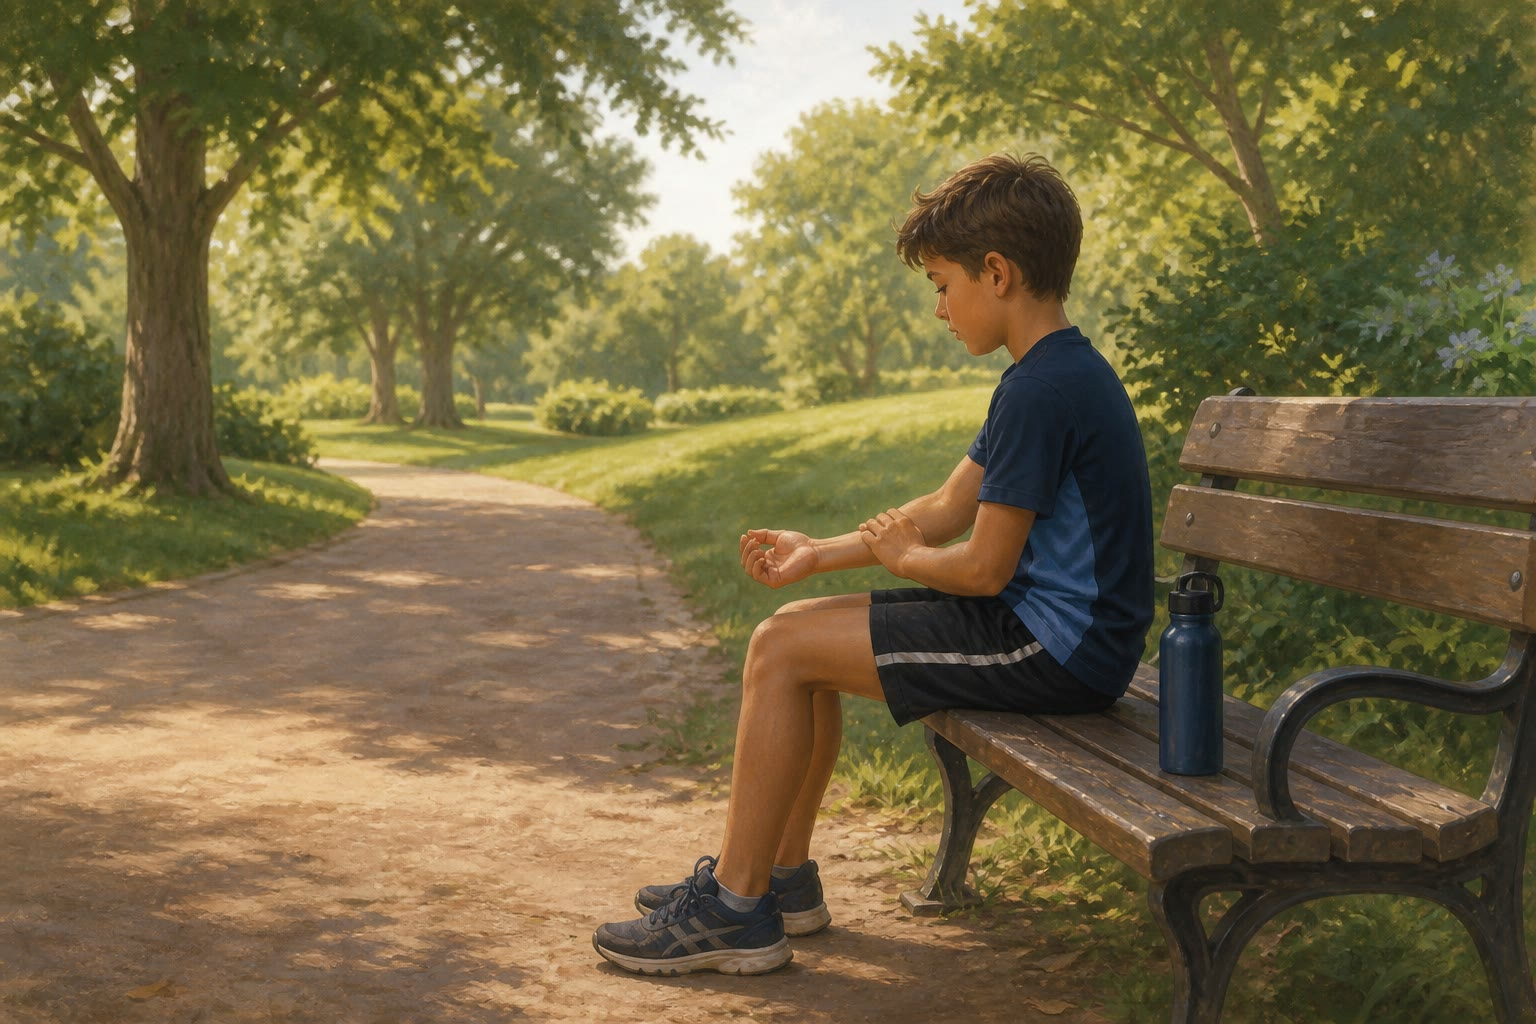
\includegraphics[width=0.58\linewidth]{images/book1/ai/g4-heart-rest.jpg}

{\small दौड़ के बाद: \omterm{def:g1:my-body:joint}{कलाई} पर दो उँगलियाँ, और दूर से \omterm{def:g4:heart-and-blood:heart}{हृदय} की दौड़ की
गिनती।}
\end{omfigure}

\begin{remark}[एक पेशी जो कभी नहीं थमती --- लगभग]\label{rem:g4:heart-and-blood:rest}
दो धड़कनों के बीच \omterm{def:g4:heart-and-blood:heart}{हृदय} सेकंड के किसी अंश भर ढीला पड़ता है --- उतना-सा
ही आराम वह कभी लेता है। दिन-रात, रोज़ लगभग $100000$ धड़कनें, पूरी उम्र
भर। हर \omterm{def:g3:bones-and-muscles:muscle}{पेशी} की तरह (\cref{met:g3:bones-and-muscles:care}) वह भी क़सरत
से मज़बूत होता है: सधा हुआ \omterm{def:g4:heart-and-blood:heart}{हृदय} हर \omterm{def:g4:heart-and-blood:heart}{धड़कन} में ज़्यादा \omterm{prop:g4:journey-of-food:absorb}{रक्त} हिलाता है,
और इसलिए ज़्यादा इत्मीनान से धड़क सकता है।
\end{remark}

\section{अभ्यास}

\begin{exercise}[$\star$]\label{exo:g4:heart-and-blood:1}
\omterm{prop:g4:journey-of-food:absorb}{रक्त} जो दो चीज़ें पहुँचाता है उनके नाम बताओ, और यह भी कि वह हर एक
कहाँ से बटोरता है।
\end{exercise}

\begin{exercise}[$\star$]\label{exo:g4:heart-and-blood:2}
\omterm{prop:g4:journey-of-food:absorb}{रक्त} कौन-सी कचरा गैस ले जाता है, और उसे कहाँ छोड़ता है?
\end{exercise}

\begin{exercise}[$\star$]\label{exo:g4:heart-and-blood:3}
\omterm{def:g4:heart-and-blood:heart}{हृदय} किसका बना है, वह कितना बड़ा है, और कहाँ बैठा है?
\end{exercise}

\begin{exercise}[$\star$]\label{exo:g4:heart-and-blood:4}
\omterm{def:g4:heart-and-blood:heart}{हृदय} का हर पक्ष क्या करता है?
\end{exercise}

\begin{exercise}[$\star$]\label{exo:g4:heart-and-blood:5}
\omterm{prop:g4:heart-and-blood:pulse}{नाड़ी} क्या है, और उसे गिनने से तुम्हें क्या पता चलता है?
\end{exercise}

\begin{exercise}[$\star$]\label{exo:g4:heart-and-blood:6}
\omterm{prop:g4:heart-and-blood:pulse}{नाड़ी} उँगलियों से क्यों देखनी चाहिए, अँगूठे से क्यों नहीं?
\end{exercise}

\begin{exercise}[$\star$]\label{exo:g4:heart-and-blood:7}
दौड़ के दौरान \omterm{prop:g4:heart-and-blood:pulse}{नाड़ी} क्यों दौड़ने लगती है? कहानी \omterm{def:g1:my-body:parts}{टाँगों} की \omterm{def:g3:bones-and-muscles:muscle}{पेशियों} की
नज़र से बताओ।
\end{exercise}

\begin{exercise}[$\star$]\label{exo:g4:heart-and-blood:8}
करके देखो: \cref{met:g4:heart-and-blood:pulse} से आराम की अपनी \omterm{prop:g4:heart-and-blood:pulse}{नाड़ी}
देखो, तीस सेकंड तारे-कूद करो, और फिर से देखो। दोनों संख्याएँ बताओ।
\end{exercise}

\begin{exercise}[$\star\star$]\label{exo:g4:heart-and-blood:9}
\cref{ex:g4:heart-and-blood:round} में \omterm{prop:g4:journey-of-food:absorb}{रक्त} की बूँद फेफड़ों से निकलते
समय चटक लाल है और \omterm{def:g1:my-body:parts}{टाँग} की \omterm{def:g3:bones-and-muscles:muscle}{पेशी} से निकलते समय गहरी। हर बार उसमें क्या
बदला?
\end{exercise}

\begin{exercise}[$\star\star$]\label{exo:g4:heart-and-blood:10}
\omterm{prop:g4:journey-of-food:absorb}{रक्त} तुम्हारी कक्षा के तीन अंगों को जोड़ता है: \omterm{def:g4:journey-of-food:tract}{छोटी आँत}, \omterm{def:g4:breathing:organs}{फेफड़े}, \omterm{def:g4:heart-and-blood:heart}{हृदय}।
इस जाल का चित्र बनाओ या वर्णन करो: पहुँचाने वाली सेवा में हर एक का क्या
योगदान है?
\end{exercise}

\begin{exercise}[$\star\star\star$]\label{exo:g4:heart-and-blood:11}
सधे हुए साइकिल-चालक की आराम वाली \omterm{prop:g4:heart-and-blood:pulse}{नाड़ी} $50$ हो सकती है; बिना सधे वयस्क
की $75$। \cref{rem:g4:heart-and-blood:rest} से समझाओ कि \emph{धीमा}
होने का मतलब \emph{मज़बूत} होना कैसे हो सकता है --- साइकिल-चालक की हर
\omterm{def:g4:heart-and-blood:heart}{धड़कन} क्या कर रही होगी?
\end{exercise}
